
\begin{frame}
\frametitle{Logarithmic relationships}
\begin{columns}[c]
\column{0.3\textwidth}
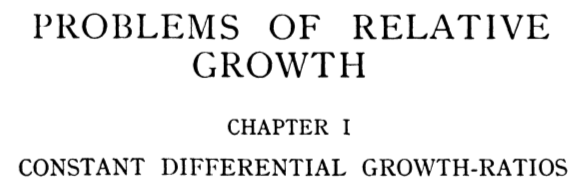
\includegraphics[width=\textwidth]{huxley}\par
\begin{tiny}
Huxley. ``Problems of relative growth.'' Methuen \& co, London (1932).\par
\end{tiny}
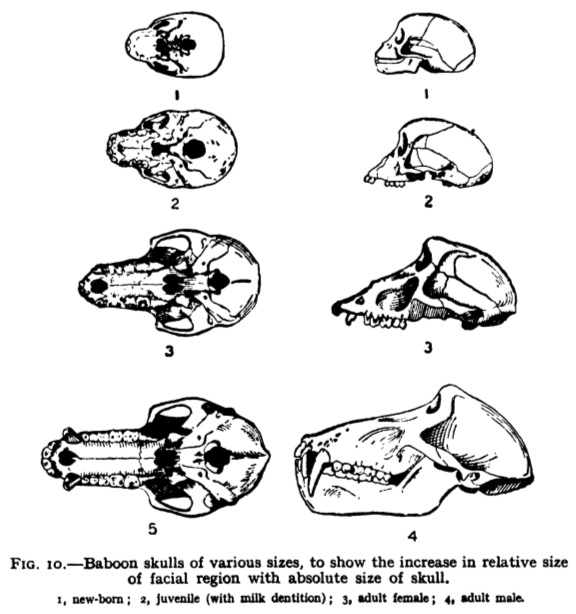
\includegraphics[width=\textwidth]{baboon_skulls}\par
\column{0.7\textwidth}
Julian Huxley demonstrated logarithmic relationships between magnitude variables (eg height, weight, length, area, volume).\par
\begin{Large}
\begin{align*}
\log y = a \log x + \log k
\end{align*}
\end{Large}
\emph{\small{``the logarithmic method
of plotting brings into true relief an important point which
is entirely obscured by the usual method of plotting on the
absolute scale -- namely the fact that growth is concerned
essentially with the multiplication of living substance.''\par}}
\end{columns}
\end{frame}


%\begin{frame}
%\frametitle{Logarithmic relationships}
%Relationships between height and weight are more linear if we take logarithms.\par
%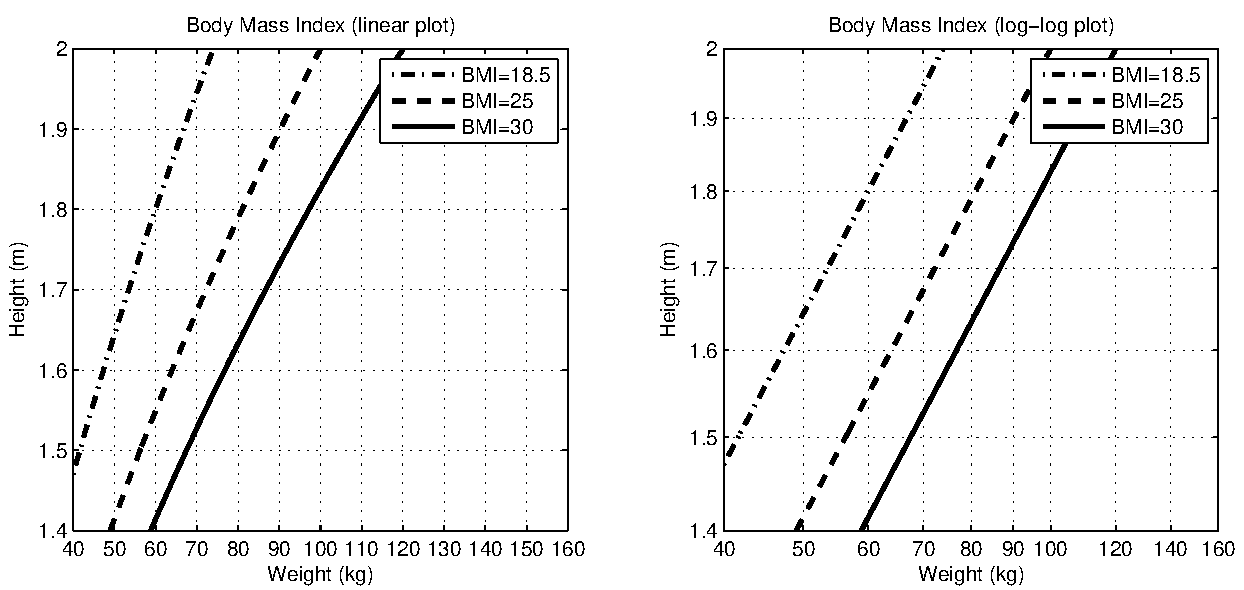
\includegraphics[width=\textwidth]{bmi}\par
%\end{frame}

\begin{frame}
\frametitle{Logarithmic relationships}
\begin{columns}[c]
\column{0.3\textwidth}
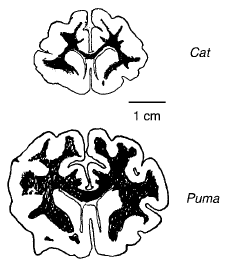
\includegraphics[width=\textwidth]{zhang_sejnowski1}\par
\column{0.7\textwidth}
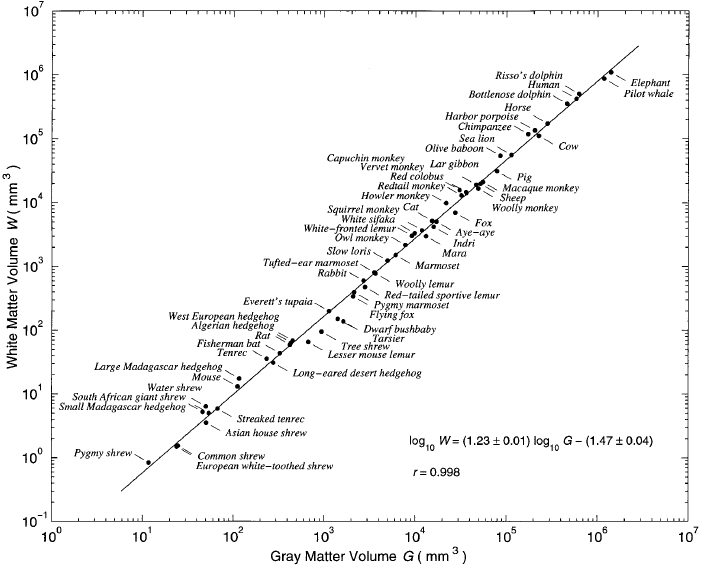
\includegraphics[width=\textwidth]{zhang_sejnowski}\par
\end{columns}
\begin{tiny}
Zhang and Sejnowski. ``A universal scaling law between gray matter and white matter of cerebral cortex.'' Proceedings of the National Academy of Sciences 97(10):5621--5626 (2000).\par
\end{tiny}
\end{frame}

\begin{frame}
\frametitle{Logarithmic relationships}
\begin{columns}[c]
\column{0.7\textwidth}
Preprocess to obtain features that behave more linearly.
%\begin{itemize}
%\item Linear methods are more interpretable.
%\item Nonlinear methods usually increase dimensionality.
%\item Better to preprocess to obtain features that behave more linearly.
%\end{itemize}
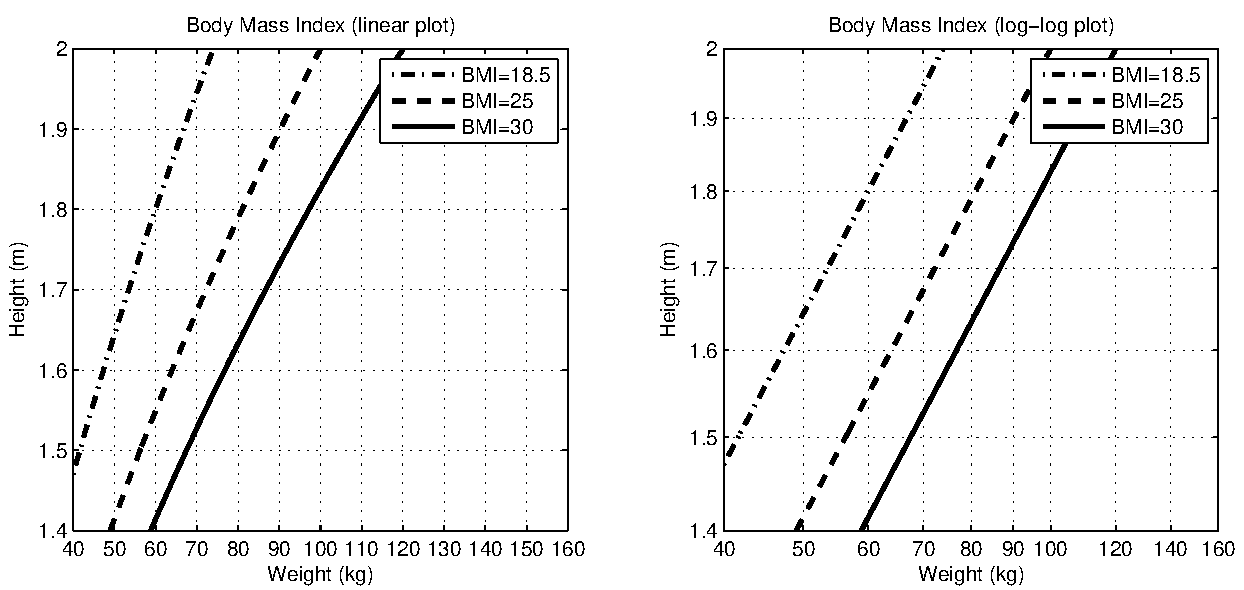
\includegraphics[width=\textwidth]{bmi}
\column{0.3\textwidth}
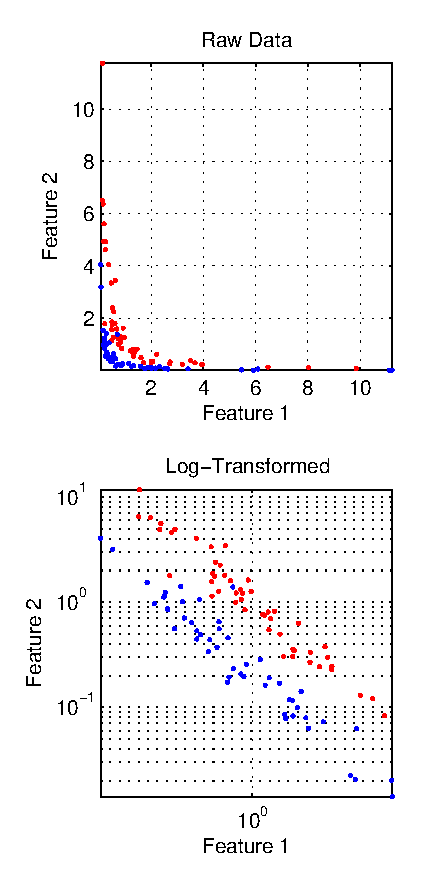
\includegraphics[width=\textwidth]{log_transformed}
\end{columns}
\end{frame}

\begin{frame}
\frametitle{Exponentials}
There are many types of exponentials and their inverses.
\end{frame}

